\begin{frame}{4. L'apprentissage profond}
  \begin{itemize}
  \item \textbf{Deep Learning} = \textit{Réseaux de Neurones} (avec plus d'une couche cachée)
  \item Conceptualisés dans les années 80 et début 90, l'explosion de la puissance de calcul disponibles a rendu possible leur exploitation
  \item \textbf{Qu'est ce que ça a à voir avec le cerveaux?} Pas grand chose en fait ... à part une analogie avec la structure des neurones
  \end{itemize}
\end{frame}

\begin{frame}{4. L'apprentissage profond}
  \begin{itemize}
  \item Utilisé principalement dans le cadre de l'\textbf{apprentissage supervisé}
    \begin{itemize}
      \normalsize
    \item Image classifiers, Object detection
    \item Speech recognition
    \item Machine traduction (\href{https://www.deepl.com/translator}{\color{blue}{DeepL}})
    \item Voiture autonomes
    \item $\dots$
    \end{itemize}
  \item Données structurées/non-structurées:
    \begin{itemize}
      \normalsize
    \item Les humains sont bons pour interpréter des données non-structurées
    \end{itemize}
  \end{itemize}
\end{frame}

\begin{frame}{4. L'apprentissage profond}
  \begin{figure}
    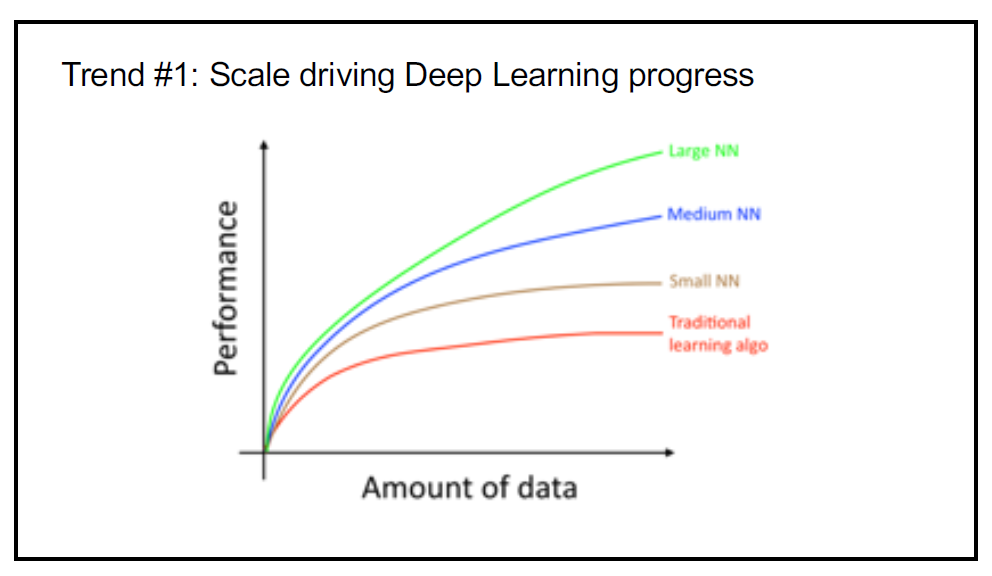
\includegraphics[width=0.8\textwidth]{fig/dataPerfAlgo.PNG}
  \end{figure}
  \vspace{-1cm}
  \begin{center}
    \footnotesize
    \textcolor{green}{Large NN}, \textcolor{blue}{Medium NN}, \textcolor{brown}{Small NN}, \textcolor{red}{Traditional learning algo}\\
    \vspace{0.1cm}
    \scriptsize
    Depuis \href{https://www.coursera.org/specializations/deep-learning}{\color{blue}{deeplearning.ai coursera}}
  \end{center}
\end{frame}
  
\begin{frame}{4.1 Les réseaux neurones}
  \begin{itemize}
  \item 1 input layer $\Rightarrow$  $L-1$ hidden layer $\Rightarrow$ 1 output layer
  \item $n^{[l]}$ cellules (neurones) pour la couche $l$, $m$ variables (input layer: $n^{[0]}$)
  \item $W^{[l]}, b^{[l]}$: paramètres de la couche $l$ ($W^{[l]} \in \mathbb{R}^{(n^{[l]} \times n^{[l-1]})}$, $b^{[l]} \in \mathbb{R}^{(n^{[l]} \times 1)}$)
  \end{itemize}
  \begin{figure}
    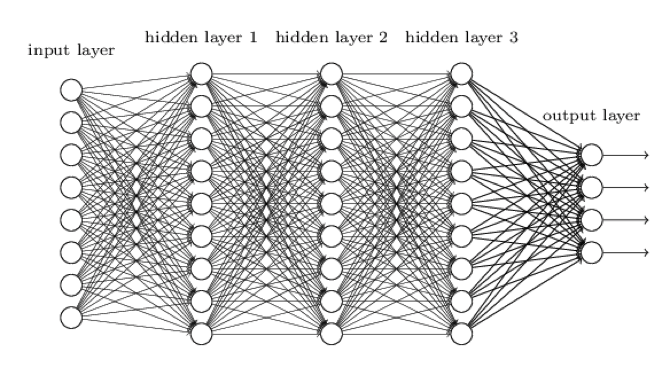
\includegraphics[width=0.6\textwidth]{fig/deepNN.png}
  \end{figure}
\end{frame}

\begin{frame}{4.1 Un neurone $i$ de la couche $l$}
  \begin{figure}
    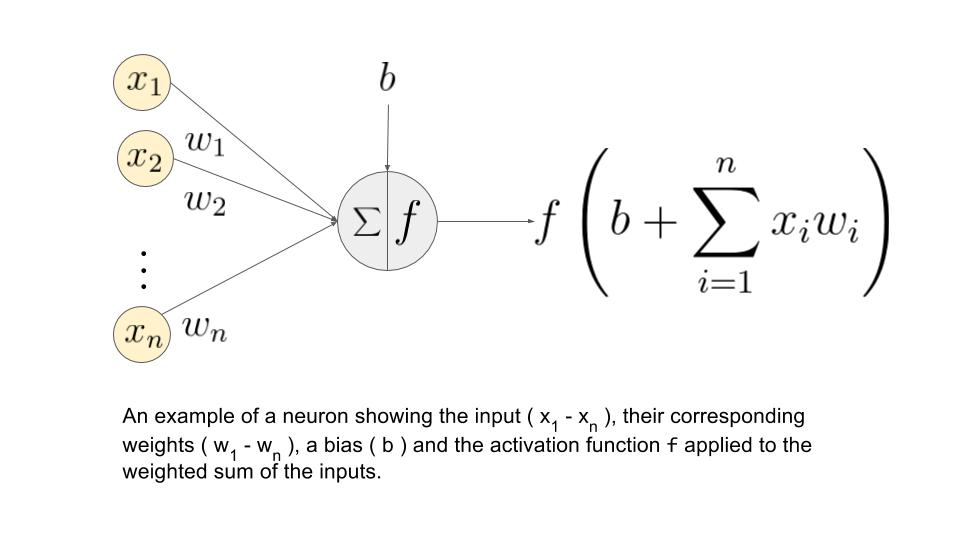
\includegraphics[trim={2cm 6cm 2cm 1.8cm},clip,width=0.7\textwidth]{fig/neuronEx.jpg}
  \end{figure}
  \begin{itemize}
  \item 2 étapes de calculs: 
    \begin{itemize}
      \normalsize
    \item $z_{i}^{[l]} = \displaystyle\sum_{j=0}^{n^{[l-1]}} w_{ij}^{[l]} \times a_{j}^{[l-1]} + b_{i}^{[l]}$ \hspace{2cm} Où, $a^{[0]} = x$
    \item $a_{i}^{[l]} = f^{[l]}(z_{i}^{[l]})$ \hfill Où, $f^{[l]}(z)$ est la \textbf{fonction d'activation}
    \end{itemize}
  \end{itemize}
\end{frame}

\begin{frame}{4.1 Une couche $l$ de neurones}
  \begin{itemize}
  \item On répète l'opération pour chaque neurone $i$ de la couche $l$
  \item Plus efficace de réfléchir en multiplication de matrices:
  \end{itemize}
  \begin{equation*}
    z^{[l]} = \begin{bmatrix*} z_{1}^{[l]} \\ z_{2}^{[l]} \\ \vdots \\ a_{n^{[l]}}^{[l]} \end{bmatrix*} = \begin{bmatrix*} w_{11}^{[l]} & w_{12}^{[l]} & \dots & w_{1n^{[l-1]}}^{[l]} \\ w_{21}^{[l]} & w_{22}^{[l]} & \dots & w_{2n^{[l-1]}}^{[l]} \\ & & \ddots & \\ w_{n^{[l]}1}^{[l]} & w_{n^{[l]}2}^{[l]} & \dots & w_{n^{[l]}n^{[l-1]}}^{[l]} \end{bmatrix*} \begin{bmatrix*} a_{1}^{[l-1]} \\ a_{2}^{[l-1]} \\ \vdots \\ a_{n^{[l-1]}}^{[l-1]} \end{bmatrix*} + \begin{bmatrix*} b_{1}^{[l]} \\ b_{2}^{[l]} \\ \vdots \\ b_{n^{[l]}}^{[l]} \end{bmatrix*}
  \end{equation*}
  \begin{itemize}
  \item Que l'on réécrira: \boldmath $z^{[l]} = W^{[l]} a^{[l-1]} + b^{[l]}$
  \item Puis: \boldmath $a^{[l]} = f^{[l]}(z^{[l]})$
  \end{itemize}
\end{frame}

\begin{frame}{4.1 Tous les exemples à la fois}
  \begin{itemize}
  \item On a vu le cas avec un exemple, mais si on veux faire les $m$ exemples en une fois? \texttt{for-loop}? $\Rightarrow$ \textbf{Matrices}!
  \item On vectorise: $X \in \mathbb{R}^{n \times m}$, plus généralement: $A^{[l]} (Z^{[l]}) \in \mathbb{R}^{n^{[l]} \times m }$
  \end{itemize}
  \begin{equation*}
    A^{[l]} = \begin{bmatrix*} a_{1}^{[l](1)} & a_{1}^{[l](2)} & \dots & a_{1}^{[l](m)}\\ a_{2}^{[l](1)} & a_{2}^{[l](2)} & \dots & a_{2}^{[l](m)}\\ & & \ddots & \\ a_{n^{[l]}}^{[l](1)} & a_{n^{[l]}}^{[l](2)} & \dots & a_{n^{[l]}}^{[l](m)}\\  \end{bmatrix*}
  \end{equation*}
  \begin{itemize}
  \item Les étapes de calculs s'écrivent: \boldmath $Z^{[l]} = W^{[l]} A^{[l-1]} + b^{[l]}$
  \item Puis: \boldmath $A^{[l]} = f^{[l]}(Z^{[l]})$
  \end{itemize}
\end{frame}

\begin{frame}{4.1 Les 4 principales fonctions d'activations}
  \begin{minipage}{0.48\textwidth}
    \begin{itemize}
    \item \textbf{Logistique:}
    \end{itemize}
    \vspace{-0.5cm}
    \begin{figure}
      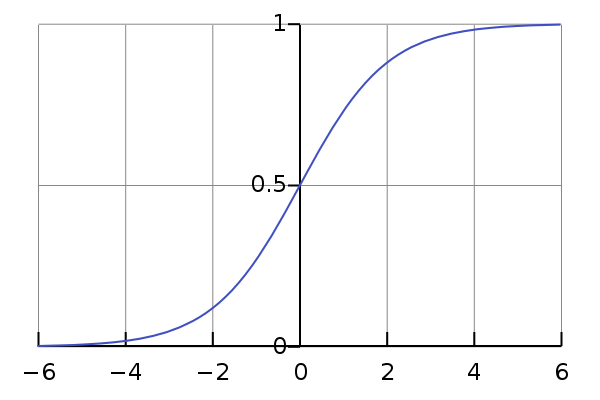
\includegraphics[width=0.8\textwidth,height=0.3\textheight]{fig/logisticFct.png}
    \end{figure}
  \end{minipage}
  \begin{minipage}{0.48\textwidth}
    \begin{itemize}
    \item \textbf{Tangente-hyperbolique:}
    \end{itemize}
    \vspace{-0.5cm}
    \begin{figure}
      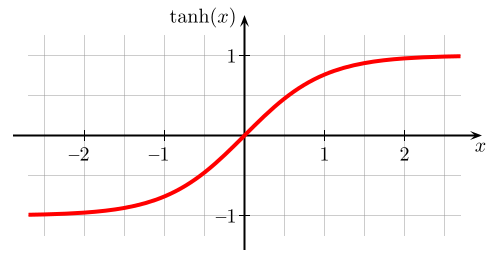
\includegraphics[width=0.8\textwidth,height=0.3\textheight]{fig/tanhFct.png}
    \end{figure}
  \end{minipage}
  \vfill
  \begin{minipage}{0.48\textwidth}
    \begin{itemize}
    \item \textbf{Rectified Linear Unit:}
    \end{itemize}
    \vspace{-0.2cm}
    \begin{figure}
      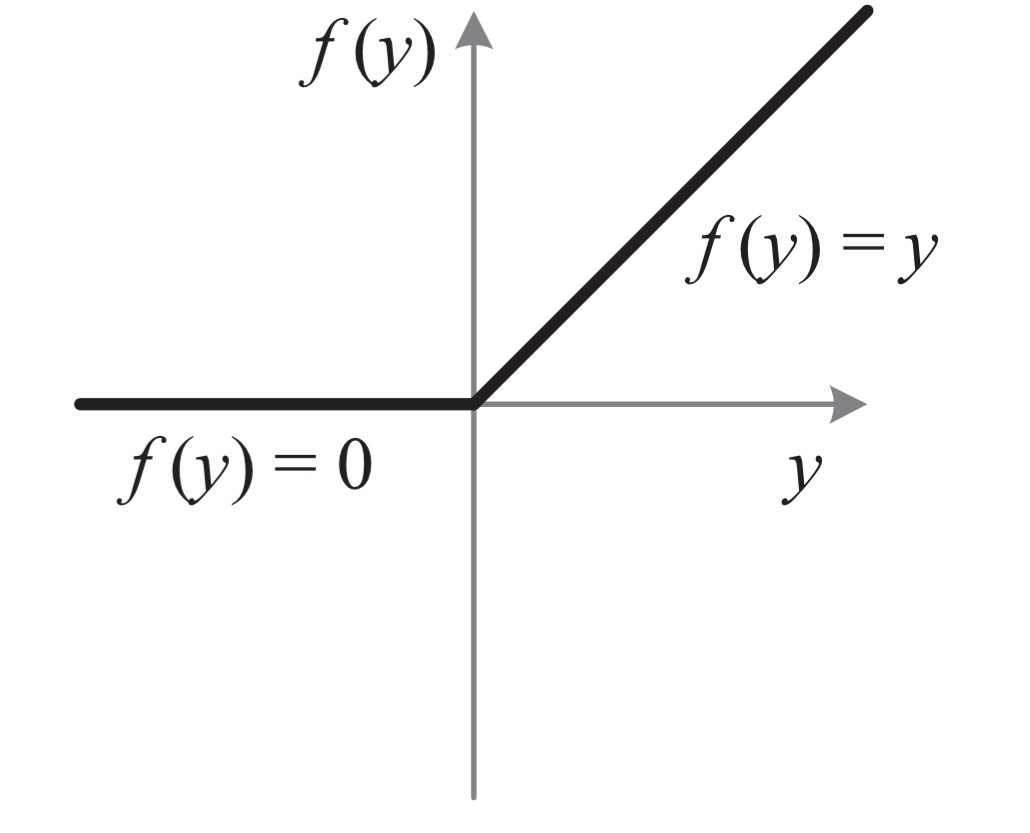
\includegraphics[width=0.8\textwidth,height=0.3\textheight]{fig/reluFct.jpeg}
    \end{figure}
  \end{minipage}
  \begin{minipage}{0.48\textwidth}
    \begin{itemize}
    \item \textbf{Leaky ReLU:}
    \end{itemize}
    \vspace{-0.5cm}
    \begin{figure}
      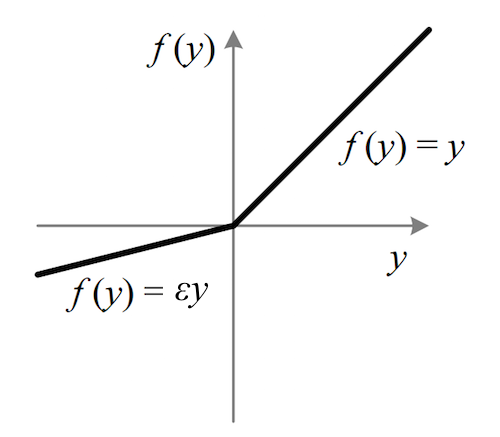
\includegraphics[width=0.8\textwidth,height=0.3\textheight]{fig/leakyReluFct.png}
    \end{figure}
  \end{minipage}
  \begin{itemize}
  \item Si $\hat{y} \in \{0,1\}$: \textbf{Logistique}. Les autres neurones: \textbf{ReLU}
  \end{itemize}
\end{frame}

\begin{frame}{4.1 Forward propagation}
  \begin{minipage}{0.62\textwidth}
    \begin{itemize}
    \item \textcolor{red}{Input \boldmath $X$ \unboldmath}: 3 variables ($n^{[0]} = 3$)
    \item \textcolor{blue}{2 couches cachées} ($n^{[1]} = n^{[2]} = 4$): \textbf{ReLU}
    \item \textcolor{forestGreen}{Output}: $n^{[3]} = 1$: \textbf{Logistique}
    \end{itemize}
  \end{minipage}
  \begin{minipage}{0.36\textwidth}
    \begin{figure}
      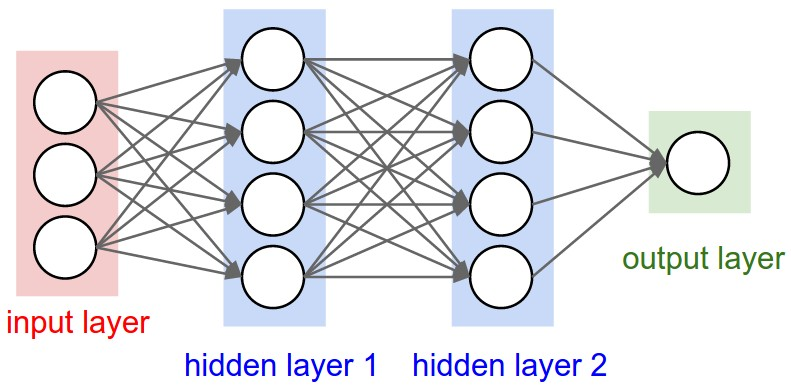
\includegraphics[width=1.0\textwidth]{fig/threelayerNN.jpg}
      \put(-120, -5){\vector(1, 0){120}}
      \put(-90, -10){\tiny \textbf{Forward propagation}}
    \end{figure}
  \end{minipage}
  \vfill
  \begin{minipage}{0.59\textwidth}
    \begin{equation*}
      \begin{matrix*}[l]
        X & \in & \mathbb{R}^{3 \times m} & & Y & \in & \mathbb{R}^{1 \times m}\\
        W^{[1]} & \in & \mathbb{R}^{4 \times 3} & & b^{[1]} & \in & \mathbb{R}^{4 \times 1}\\
        Z^{[1]} & \in & \mathbb{R}^{4 \times m} & & A^{[1]} & \in & \mathbb{R}^{4 \times m}\\
        W^{[2]} & \in & \mathbb{R}^{4 \times 4} & & b^{[2]} & \in & \mathbb{R}^{4 \times 1}\\
        Z^{[2]} & \in & \mathbb{R}^{4 \times m} & & A^{[2]} & \in & \mathbb{R}^{4 \times m}\\
        W^{[3]} & \in & \mathbb{R}^{1 \times 4} & & b^{[3]} & \in & \mathbb{R}^{1 \times 1}\\
        Z^{[3]} & \in & \mathbb{R}^{1 \times m} & & A^{[3]} & \in & \mathbb{R}^{1 \times m}\\
      \end{matrix*}
    \end{equation*}
  \end{minipage}
  \begin{minipage}{0.39\textwidth}
    \begin{equation*}
      \begin{matrix*}[l]
        Z^{[1]} = W^{[1]} X + b^{[1]}\\
        A^{[1]} = f^{[1]}(Z^{[1]}) = relu(Z^{[1]})\\
        Z^{[2]} = W^{[2]} A^{[1]} + b^{[2]}\\
        A^{[2]} = f^{[2]}(Z^{[2]}) = relu(Z^{[2]})\\
        Z^{[3]} = W^{[3]} A^{[2]} + b^{[3]}\\
        \hat{Y} = A^{[3]} = f^{[3]}(Z^{[3]}) = \sigma(Z^{[3]})\\
      \end{matrix*}
    \end{equation*}
  \end{minipage}
\end{frame}

\begin{frame}{4.1 Backward propagation}
  \begin{itemize}
  \item C'est l'algorithme d'\textit{apprentissage} des réseaux de neurones
  \item On définit la fonction de coût:
  \end{itemize} 
  \begin{equation*}
    J(W^{[1]},\dots,W^{[L]},b^{[1]},\dots,b^{[L]}) = \frac{1}{m}\displaystyle\sum_{i=1}^{m}L(\hat{y}^{(i)},y^{(i)})
  \end{equation*}
  \vspace{-0.5cm}
  \begin{itemize}
  \item On utilise la \textbf{descente de gradient}:
  \end{itemize}
  \begin{equation*}
    \begin{matrix*}[l]
      \text{Répéter:} & \{ & \\ & & \text{Calculez: } \hat{Y} \\ & & dW^{[L]} := \frac{dJ}{dW^{[L]}}, ~~ db^{[L]} := \frac{dJ}{db^{[L]}}\\ & & W^{[L]} := W^{[L]} - \alpha dW^{[L]} \\ & & b^{[L]} := b^{[L]} - \alpha db^{[L]} \\ & & \vdots \\ & \} &
    \end{matrix*}
  \end{equation*}
\end{frame}


\begin{frame}{4.1 Backward propagation}
  \begin{itemize}
  \item On va propager l'erreur $\hat{Y} - Y$ pour modifier les valeurs des paramètres $W^{[l]}$ et $b^{[l]}$ du réseau de neurones
  \end{itemize}
  \begin{minipage}{0.36\textwidth}
    \begin{figure}
      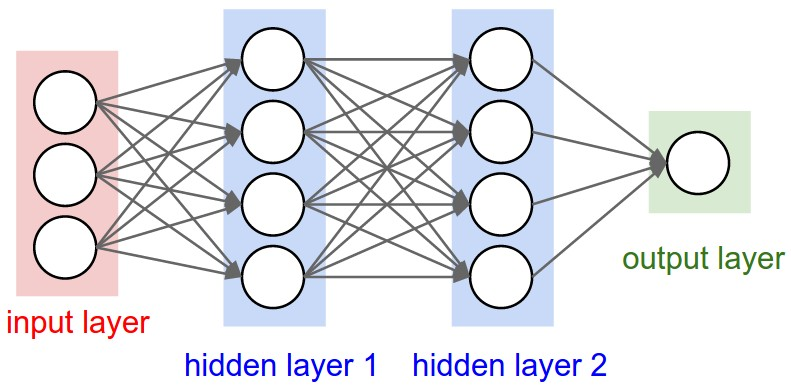
\includegraphics[width=1.0\textwidth]{fig/threelayerNN.jpg}
      \put(0, -5){\vector(-1, 0){120}}
      \put(-90, -10){\tiny \textbf{Backward propagation}}
    \end{figure}
  \end{minipage}
  \begin{minipage}{0.62\textwidth}
    \begin{equation*}
      \begin{matrix*}[l]
        dZ^{[3]} = A^{[3]} - Y\\
        dW^{[3]} = \frac{1}{m} dZ^{[3]} A^{[2]}{}^{T}\\
        db^{[3]} = \frac{1}{m}\sum dZ^{[3]} \\
        dZ^{[2]} = W^{[3]}{}^{T} dZ^{[3]} * relu'(Z^{[2]})\\
        dW^{[2]} = \frac{1}{m} dZ^{[2]} A^{[1]}{}^{T}\\
        db^{[2]} = \frac{1}{m}\sum dZ^{[2]} \\
        dZ^{[1]} = W^{[2]}{}^{T} dZ^{[2]} * relu'(Z^{[1]})\\
        dW^{[1]} = \frac{1}{m} dZ^{[1]} X^{T}\\
        db^{[1]} = \frac{1}{m}\sum dZ^{[1]} \\
      \end{matrix*}
    \end{equation*}
  \end{minipage}
  \vspace{0.5cm}
  \begin{itemize}
  \item Pour que l'apprentissage fonctionne: \textbf{Initialisation aléatoire} $W,b$
  \end{itemize}
\end{frame}

\begin{frame}{4.2 Les bonnes pratiques: préparer les donneés}
  \begin{itemize}
  \item On sépare les données en trois sous-échantillons:
    \begin{itemize}
      \normalsize
    \item \textbf{Train:} (60$\%$) échantillon d'entrainement avec lequel on applique la \textit{forward-backward propagation}
    \item \textbf{Validation:} (20$\%$) échantillon qui nous permet de mesurer les performances du modèle pour différentes valeurs d'hyperparamètres et différentes architectures
    \item \textbf{Test:} (20$\%$) échantillon de test qui donne la performance du modèle final
    \end{itemize}
  \item Il est important de séparer les données en différents sous-échantillons de test pour être sûr que le modèle de généralise bien
  \item S'assurer que les sous-échantillons proviennent de la même source et soient représentatifs
  \end{itemize}
\end{frame}

\begin{frame}{4.2 Les bonnes pratiques: biais et variance}
  \begin{itemize}
  \item Si $J_{train}(W,b) >> J_{valid}(W,b)$: problème de variance: \textbf{Overfitting}
  \item Si $J_{train}(W,b) \approx J_{valid}(W,b) >> 0$: problème de biais: \textbf{Underfitting}
  \item Comment diagnostiquer? deux valeurs à regarder:
    \begin{itemize}
      \normalsize
    \item Erreur de l'échantillon d'entrainement: $t_{err}$
    \item Erreur de l'échantillon de validation: $v_{err}$
    \end{itemize}
  \item On estime le cas idéal (Bayes ou opérateur humain): $\approx 0\%$
  \end{itemize}
  \vspace{0.5cm}
  \begin{minipage}{.39\textwidth}
    \begin{figure}
      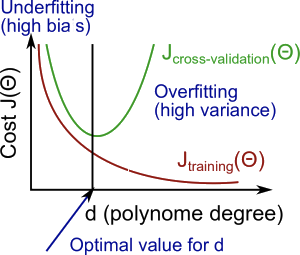
\includegraphics[trim={0 54 0 0},clip,width=\textwidth]{fig/biasVsVariance}
    \end{figure}
    \vspace{-1cm}
    \begin{center}
      \scriptsize
      \href{https://www.coursera.org/learn/machine-learning}{\color{blue}{[Coursera]}}
    \end{center}
  \end{minipage}
  \begin{minipage}{.59\textwidth}
    \begin{table}
      \begin{tabular}{l|l|l}
        $t_{err}$ & $v_{err}$ & problème \\
        \hline
        1$\%$ & 11$\%$ & haute variance \\
        15$\%$ & 16$\%$ & haut biais \\
        15$\%$ & 30$\%$ & haut biais \& haute variance \\
        0.5$\%$ & 1$\%$ & bas biais \& basse variance \\
      \end{tabular}
    \end{table}
  \end{minipage}
\end{frame}

\begin{frame}{4.2 Les bonnes pratiques: courbes d'apprentissage}
  \begin{itemize}
  \item Entrainer un algo en augmentant le nombre d'exemples et monitorer l'évolution de l'erreur:
  \end{itemize}
  \begin{figure}
    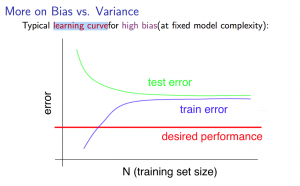
\includegraphics[trim = {0 0 0 32}, clip, width=0.44\textwidth]{fig/learningCurves1.png}
    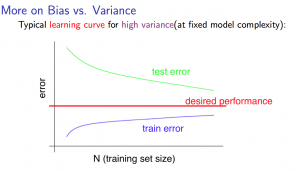
\includegraphics[trim = {0 0 0 30}, clip, width=0.48\textwidth]{fig/learningCurves2.png}
  \end{figure}
  \vspace{-0.5cm}
  \begin{center}
    \scriptsize
    Biais et variance \href{https://www.coursera.org/learn/machine-learning}{\color{blue}{[Coursera]}}
  \end{center}  
\end{frame}

\begin{frame}{4.2 Les bonnes pratiques: Que faire?}
  \begin{table}
    \footnotesize
    \begin{tabular}{ccccl}
      \multicolumn{3}{l}{\textcolor{orange}{\textbf{$\bullet$ Haut Biais?}}} & \boldmath $\rightarrow$ \textbf{Oui} $\rightarrow$ \unboldmath & Réseau plus profond \\
      \multicolumn{3}{l}{(Performance entrainement)} & & Entrainer plus longtemps \\
      & & & & Changer architecture du NN \\
      & & \boldmath $\downarrow$ \unboldmath & & \multicolumn{1}{c}{\boldmath $\downarrow$ \boldmath} \\
      & & \textbf{Non} & & \multicolumn{1}{c}{\textit{\textcolor{orange}{Recommencer!}} \boldmath $\rightarrow$ \unboldmath}\\
      & & \boldmath $\downarrow$ \unboldmath & & \\
      & & & & \\
      \multicolumn{3}{l}{\textcolor{orange}{\textbf{$\bullet$ Haute Variance?}}} & \boldmath $\rightarrow$ \textbf{Oui} $\rightarrow$ \unboldmath & Plus de données \\
      \multicolumn{3}{l}{(Performance validation)} & & Regularisation \\
      & & & & Changer architecture du NN \\
      & & \boldmath $\downarrow$ \unboldmath & & \multicolumn{1}{c}{\boldmath $\downarrow$ \boldmath} \\
      & & \textbf{Non} & & \multicolumn{1}{c}{\textit{\textcolor{orange}{Recommencer!}} \boldmath $\rightarrow$ \unboldmath}\\
      & & \boldmath $\downarrow$ \unboldmath & & \\
      & & & & \\
      & & \textcolor{orange}{\textbf{OK!}} & & \\      
    \end{tabular}
  \end{table}
\end{frame}

\begin{frame}{4.3 Les différentes architectures de NN}
  \begin{itemize}
  \item Différentes architectures pour différents usages:
  \end{itemize}
  \vspace{0.5cm}
  \footnotesize
  \begin{minipage}{.3\textwidth}
    \begin{center}
      \textbf{\textcolor{orange}{Std NN}}
    \end{center}
    \begin{figure}
      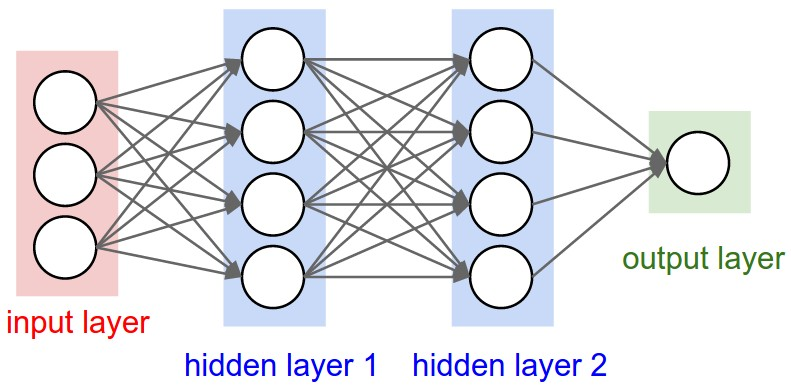
\includegraphics[width=0.9\textwidth,height=0.2\textheight]{fig/threelayerNN.jpg}
    \end{figure}
    Regression\\
    Classification\\
  \end{minipage} 
  \begin{minipage}{.3\textwidth}
    \begin{center}
      \textbf{\textcolor{orange}{Convolutional NN}}
    \end{center}
    \begin{figure}
      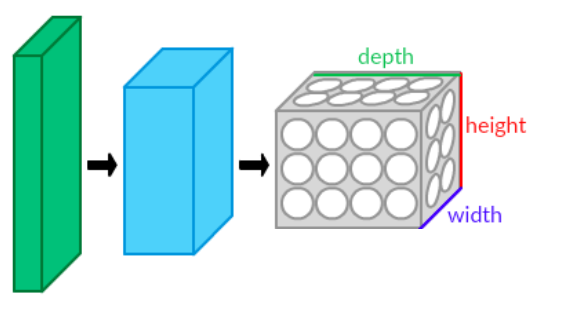
\includegraphics[width=0.9\textwidth,height=0.2\textheight]{fig/CNN.png}
    \end{figure}
    Image classifier\\
    Object detection\\
  \end{minipage}  
  \begin{minipage}{.3\textwidth}
    \begin{center}
      \textbf{\textcolor{orange}{Recurent NN}}
    \end{center}
    \begin{figure}
      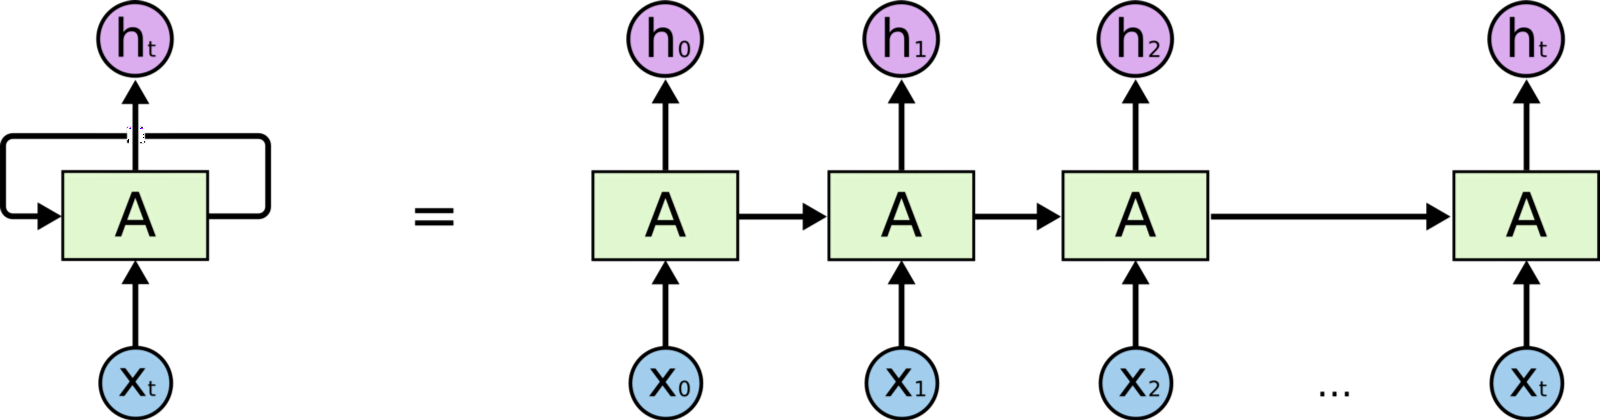
\includegraphics[width=0.9\textwidth,height=0.2\textheight]{fig/RNN.png}
    \end{figure}
    Audio recognition\\
    Time Series analysis\\
  \end{minipage}
\end{frame}

